\section{Preprocessing Top-Level Forms}

Having defined and explained transformation/analysis passes for both patterns and term-templates, these are combined according to the needs of top-level forms. They are depicted in Figure \ref{transform-pipeline}. 

There are three different strategies that can be applied to patterns. Strategy \textbf{(a)} is applied to all patterns used in \texttt{define-language} form. Strategy \textbf{(b)} is applied to patterns used for domain/codomain testing of terms. Strategy \textbf{(c)} is applied to any other pattern. For term-templates, there's only a single transformation strategy.

\begin{figure}[ht]
\centering
	\makebox[\textwidth][c] { 
		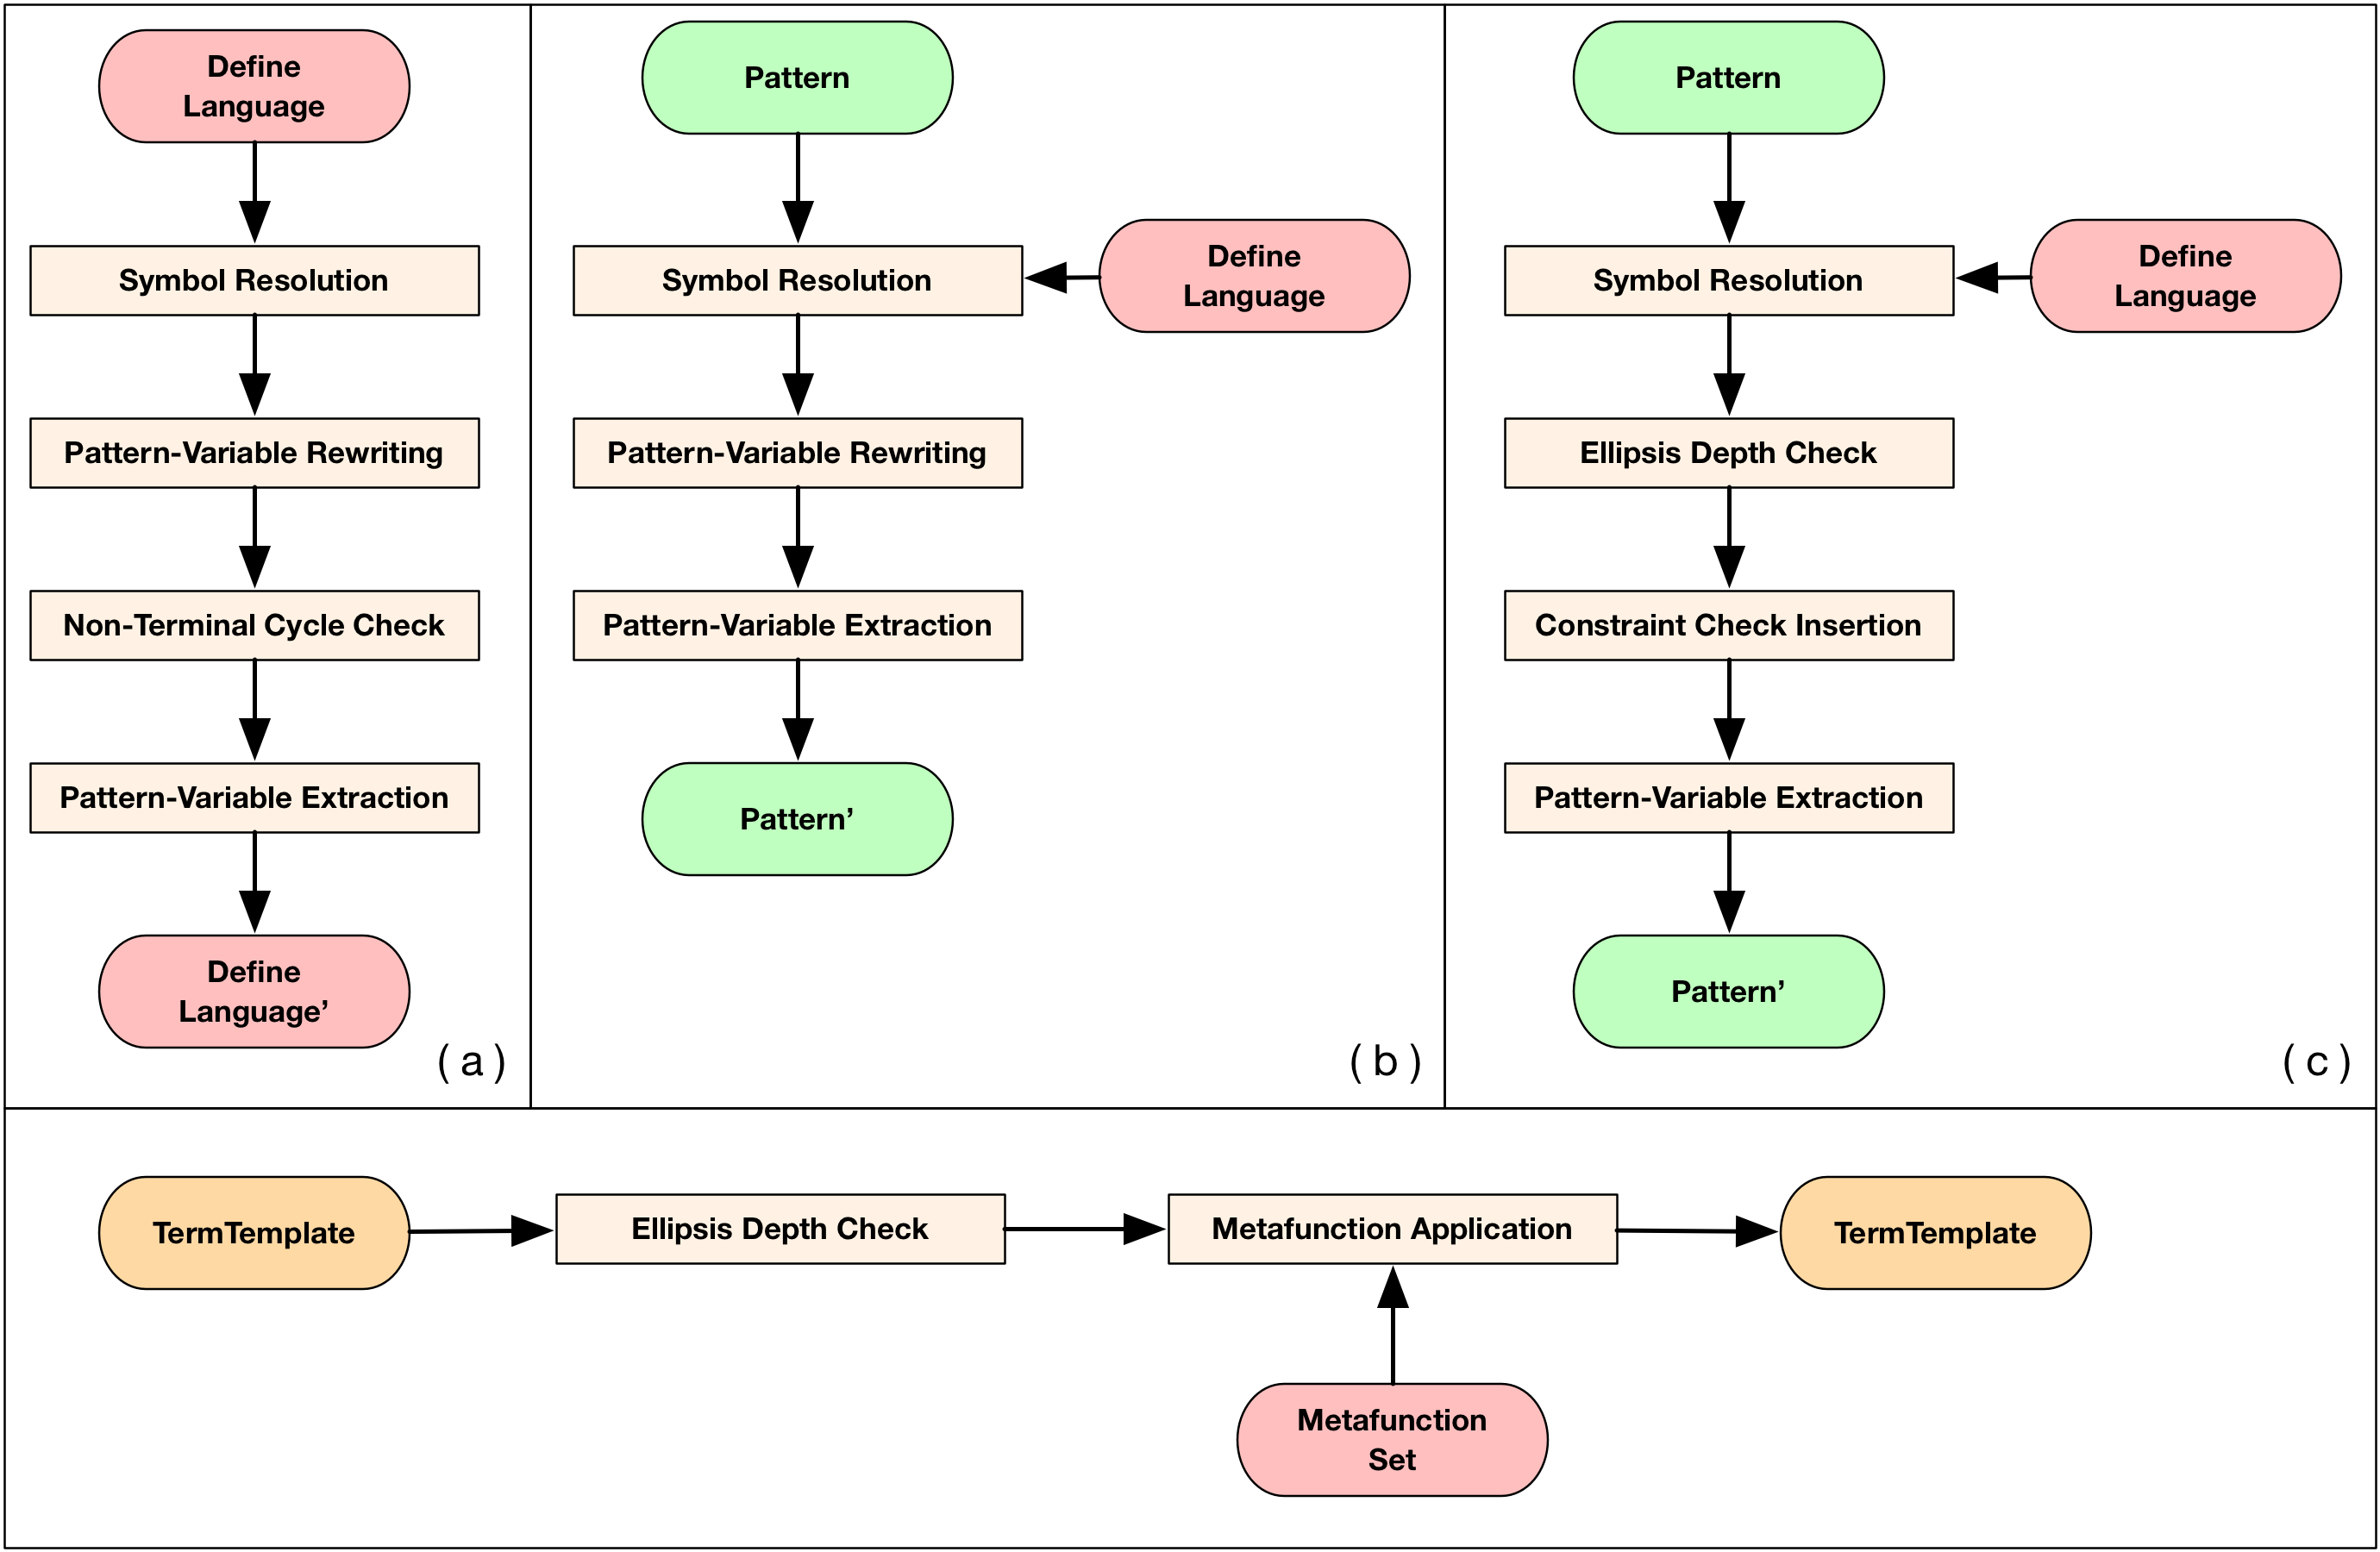
\includegraphics[scale=0.165]{transform-pipeline.png}
	}
	\caption{Transformations applied to patterns and term-templates.}
	\label{transform-pipeline}
\end{figure}


Notice that non-terminal resolution occurs with respect to non-terminal definitions on some \DefineLanguageNoArg \space form. Similarly, \textit{Metafunction Application} Pass requires the set $Mf$ containing all meta-functions defined until this point. 

\begin{enumerate}
\item All $tl=$\space \TlDefineLanguage \space forms. Maintain a set $L$ that stores ($n, tl$) pairs.
\item All $tl=$\space \TlDefineMetafunction \space forms. Maintain a set $M$ that stores $(n, tl)$ pairs.
\item All $tl=$\space \TlDefineReductionRelation \space forms. Maintain a set $R$ that contains $(n, tl)$ pairs.
\end{enumerate}

\subsection{Top-Level Form Analysis}

\begin{itemize}
\item
Given $tl=$\space \TlDefineLanguage
	\begin{enumerate}
		\item Apply strategy \textbf{(a)} to $tl$ resulting in $tl^{\prime}$.
		\item $L = L \cup \{ (n, tl^{\prime}) \}$
		\item Return $tl^{\prime}$.
	\end{enumerate}

\item $tl=$\space \TlDefineMetafunction:
	\begin{enumerate}
	\item Ensure that there exists a tuple $(l, df) \in L$, otherwise raise an Exception.
	\item Apply strategy \textbf{(b)} to $domain$ and $codomain$ patterns resulting in $domain^\prime$ and $codomain^\prime$.
	\item For each $mc_i=$ \MetafunctionCase, apply strategy \textbf{(c)} to $p$ thus resulting in $p^{\prime}$ and apply term-processing strategy to $t$ resulting in $t^{\prime}$. Let $mc_i^{\prime}$ = \MetafunctionCase[$p^{\prime}$][$t^{\prime}$].
	\item Let $tl^\prime$  = \TlDefineMetafunction[$n$][$l$][$domain^\prime$][$codomain^\prime$][$mc_1^\prime$][$mc_n^\prime$][false].
	\item $M = M \cup \{ (n, tl^\prime)\}$ and return $tl^\prime$.
	\end{enumerate}

\item $tl=$ \TlDefineReductionRelation:
\begin{enumerate}
\item Ensure that there exists a tuple $(l, df) \in L$ otherwise raise an Exception.
\item Apply strategy \textbf{(b)} to $domain$ pattern resulting in $domain^\prime$, if it exists.
\item For each $rc_i=$ \ReductionCase \space in $r$, apply strategy \textbf{(c)} to $p$ resulting in $p^{\prime}$ and apply the only term-processing strategy to $t$ resulting in $t^\prime$. Let $rc_i^\prime=$\space \ReductionCase[$p^{\prime}$][$t^{\prime}$][$n$][false].
\item Let $tl^\prime=$\space \TlDefineReductionRelation[$n$][$l$][$domain^\prime$][$rc_1^\prime$][$rc_n^\prime$]
\item $R = R \cup \{ (n, tl^\prime) \}$ and return $tl^\prime$.

\end{enumerate}

\item $tl=$ \ReadFromStdinAndApplyReductionRelation
\begin{enumerate}
\item If $f$ is present, ensure there exists a tuple $(f, mf) \in M$, otherwise raise Exception.
\item Ensure there exists a tuple $(r, red) \in R$, otherwise raise an Exception.
\item Return $tl$.
\end{enumerate}

\item
$tl=$ \RedexMatchAssertEqual.
	\begin{enumerate}
	\item Ensure that there exists a tuple $(l, df) \in L$, otherwise raise an Exception.
	\item Process $p$ according to strategy \textbf{(c)} resulting in $p^\prime$.
	\item Process $t$ according to the only specified strategy, resulting in $t^\prime$.
	\item For each $m_i=$\space \Match, process each $t_i$ according to the only specified strategy resulting in $t_i^\prime$. Let $m_i^\prime=$\space \Match[$s_1$][$t_1^\prime$][$s_n$][$t_n^\prime$][false].
	\item Let $tl^\prime=$\space\RedexMatchAssertEqual[$l$][$p^\prime$][$t^\prime$][$m_1^\prime$][$m_n^\prime$][false] and return $tl^\prime$.
	\end{enumerate}

\item $tl=$ \TermLetAssertEqual
	\begin{enumerate}
	\item  Process each $t_i$ according to the only specified strategy resulting in $t_i^\prime$.
	\item Process $t$ and $e$ according to the only specified strategy, resulting in $t^\prime$ and $e^\prime$, respectively.
	\item Let $tl^\prime=$\space \TermLetAssertEqual[$v_1$][$n_1$][$t_1^\prime$][$v_m$][$n_m$][$t_m^\prime$][$t^\prime$][$e^\prime$][false] and return $tl^\prime$.
	\end{enumerate}

\item $tl=$ \ApplyReductionRelationAssertEqual
	\begin{enumerate}
	\item Ensure that there exists a tuple $(r, red) \in R$, otherwise raise an Exception.
	\item Process $t$ according to the only specified strategy resulting in $t^\prime$
	\item Process each term $e_i$ according to the only specified strategy, resulting in $e_i^\prime$.
	\item Let $tl^\prime=$\space \ApplyReductionRelationAssertEqual[$r$][$t^\prime$][$e_1^\prime$][$e_n^\prime$][false] and return $tl^\prime$.
	\end{enumerate}
\end{itemize}

\subsection{Remarks}
It should be noted that the way in which PyPltRedex handles metafunction resolution is slightly different from PLTRedex. PLTRedex seems to keep track of metafunctions that have been defined up until a certain point, and it also keeps track of metafunctions that have not been defined yet. Roughly speaking, instead of passing a single set $Mf$ into "Metafunction Application Pass", PLTRedex passes a second set $\overline{Mf}$ containing names of metafunctions that haven't been defined yet. This way, when attempting to detect metafunction applications, "Metafunction Application Pass" also checks set $\overline{Mf}$ and raises \textbf{"cannot use metafunction before its definition"} error. Since PyPltRedex doesn't handle this at this time, all possible metafunction applications do not get rewritten and thus more often than not $codomain$ check fails.
